\section{Analytical results}

\subsection{Transfer orbit}
\label{sec:transfer_anal}

\begin{figure}[h]
    \centering
    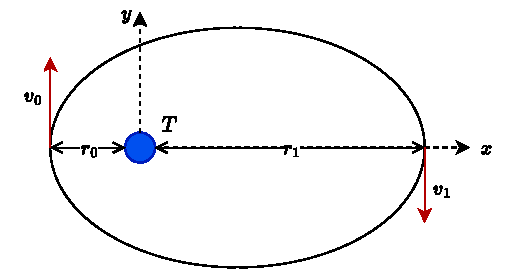
\includegraphics[width=0.6\linewidth]{figures/transfert.pdf}
    \caption{Schematic of the transfer orbit of Webb}
    \label{fig:schema_transfert}
\end{figure}
In this first part we will only consider the gravitational pull from the Earth. We would like to calculate the speed $v_0$ needed for Webb to reach a distance \(r_1 = 1.5\) million km from Earth at the peak of the transfer orbit, starting from a lower distance \(r_0 = 6800\) km as shown in \autoref{fig:schema_transfert}. Let \(m\) be the mass of Webb, \(m_T\) the mass of the Earth, \(v_0\) and \(v_1\) the required start and end speed respectively. We have that the gravitational force is central on the Earth $T$ therefore angular momentum relative to $T$ is conserved, we can thus write:
\begin{equation}
    r_0 v_0 = r_1 v_1
    \label{eq:conservation_moment_cinetique}
\end{equation}
The only force here derives from the potential $U(\vec{r}) = -G \frac{m m_T}{r}$ with $\vec{r}$ the position. Using conservation of energy:
\begin{equation}
    \frac{1}{2} m v_0^2 - G \frac{m m_T}{r_0} = \frac{1}{2} m v_1^2 - G \frac{m m_T}{r_1}
    \label{eq:conservation_energy}
\end{equation}
where \(G = 6.674 \cdot 10^{-11}\) \si{\meter\cubed\per\kilo\gram\per\second\squared} is the universal gravitational constant. Using \autoref{eq:conservation_moment_cinetique} we get:
\begin{equation}
    v_0 = \frac{r_1 v_1}{r_0}
    \label{eq:v0_substitution}
\end{equation}
which we can then substitute in \autoref{eq:conservation_energy} to get:
\begin{equation}
    \frac{1}{2} m \left(\frac{r_1}{r_0}\right)^2 v_1^2 - G \frac{m m_T}{r_0} = \frac{1}{2} m v_1^2 - G \frac{m m_T}{r_1}
\end{equation}
Solving for \(v_1\) and with $r_0 \neq r_1$ we get the following expression:
\begin{equation}
    v_1 = r_0 \sqrt{2 G m_T \frac{\frac{1}{r_0}-\frac{1}{r_1}}{r_1^2-r_0^2}}
\end{equation}
Using \autoref{eq:v0_substitution}, we have
\begin{equation}
    v_0 = r_1 \sqrt{2 G m_T \frac{\frac{1}{r_0}-\frac{1}{r_1}}{r_1^2-r_0^2}}
    \label{eq:v0_final}
\end{equation}
Evaluating these expressions using \(m_T = 5.9736 \cdot 10^{24}\) kg gives us
\begin{equation}
    v_0 \approx 10804 \, \textrm{m/s} \quad v_1 \approx 49 \, \textrm{m/s}
\end{equation}

We now want to obtain the equations of motion of Webb in this first orbit. Let us take the vector \(\mathbf{y} = (x(t), y(t), v_x(t), v_y(t))\) with $v_x(t) = \dot x(t)$ and $v_y(t) = \dot y(t)$. We are searching for \(\mathbf{f}\) such that:
\begin{equation}
    \frac{\dd \mathbf{y}}{\dd t} = \left(\begin{matrix} \dot x \\ \dot y \\ \ddot x \\ \ddot y \end{matrix}\right) = \mathbf{f}(\mathbf{y})
\end{equation}
The only force applied on Webb is the gravitational pull of the Earth $\vec{F} = -G \frac{m m_T}{r^3}\vec{r}$. The equations of motion along \(\hat{x}\) and \(\hat{y}\) are:
\begin{equation}
    \begin{cases}
        m \ddot x = -G \frac{m m_T}{\left(x^2+y^2\right)^\frac{3}{2}} x \\
        m \ddot y = -G \frac{m m_T}{\left(x^2+y^2\right)^\frac{3}{2}} y
    \end{cases}
\end{equation}
Which allows us to express \(\mathbf{f}(\mathbf{y})\) as
\begin{equation}
    \frac{\dd \mathbf{y}}{\dd t} = \mathbf{f}(\mathbf{y}) = \left(\begin{matrix} v_x \\ v_y \\ -G \frac{m_T}{\left(x^2+y^2\right)^\frac{3}{2}} x \\ -G \frac{m_T}{\left(x^2+y^2\right)^\frac{3}{2}} y \end{matrix}\right).
\end{equation}

\subsection{Sun-Earth system}

We now consider the Sun-Earth system, where \(m_S = 1.98892 \cdot 10^{30}\) kg and \hbox{\(m_T = 5.9736 \cdot 10^{24}\) kg} are the respective masses of these objects. Supposing a constant distance \(d = 149598023\) km between the Sun and the Earth and a circular orbit, we want to obtain the position of the Sun \(x_S'\) and Earth \(x_T'\) relative to their center of mass \(\mathcal G\). We position the axis \(x'\) as the Sun-Earth axis, where the center of mass \(\mathcal G\) is at \(x'=0\). This coordinate system is shown in \autoref{fig:schema_referentiel}.
\begin{figure}[h]
    \centering
    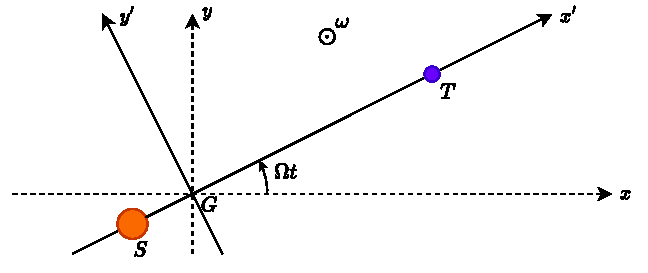
\includegraphics[width=0.8\linewidth]{figures/referentiel.pdf}
    \caption{Referential rotating along with the Earth and the Sun}
    \label{fig:schema_referentiel}
\end{figure}
Using the equation for the position of the center of mass, i.e.
\begin{equation}
    \begin{aligned}
        &\mathcal G = \frac{x_T' m_T + x_S' m_S}{m_T + m_S} \stackrel{!}{=} 0 \\
        &\implies x_T' m_T + x_S' m_S = 0
    \end{aligned}
\end{equation}
and the fact that the distance between the Sun and Earth is given by \(|x_T'|+|x_S'| = x_T' - x_S' = d\), where the minus sign is because \(x_S'\) is on the left hand side of \(\mathcal G\), we get a system of equations
\begin{equation}
    \begin{cases}
        x_T' - x_S' = d \\
        x_T' m_T = -x_S' m_S
    \end{cases}
\end{equation}
Solving this system gives us the positions of the Sun and Earth in this new coordinate system
\begin{equation}
    x_T' = \frac{m_S d}{m_T + m_S}, \quad x_S' = - \frac{m_T d}{m_T + m_S}
    \label{eq:pos_earth_sun}
\end{equation}

We would also like to know the angular speed \(\Omega\) of the planets, which have the same $\Omega$ as they move in phase. Using the circular orbit hypothesis, we get that the motion is circular uniform. This allows us to express the norm of the acceleration \(a\) as \(a = \frac{v^2}{r}\), where \(v^2\) is the squared norm of the speed of the planet and \(r\) is the radius of its orbit. Because \(v = \Omega r\), we have \(a = \Omega^2 r\). Furthermore, using \(\vec F=m \vec a \implies a = \left|\frac{F}{m}\right|\), we get for the orbit of the Earth
\begin{equation}
    \left|\frac{F}{m_T}\right| = G \frac{m_S}{d^2} = \Omega^2 x_T'
\end{equation}
which gives an expression for the angular speed \(\Omega\)
\begin{equation}
    \Omega = \sqrt{G \frac{m_S}{d^2 x_T'}} = \sqrt{G\frac{m_T + m_S}{d^3}}
\end{equation}
where only the positive root was taken because we take the motion to be counter-clockwise, as shown in \autoref{fig:schema_referentiel}. We denote the rotation vector \(\vec\Omega = (0, 0, \Omega)\). Evaluating numerically, we get \(\Omega \approx 1.99 \cdot 10^{-7}\) rad/s, which does give an orbital period \(T = \frac{2 \pi}{\Omega} \approx 365.2\) days as expected.

\subsection{Equations of motion in rotating frame of reference}
\label{sec:3body_reduced}

Let \(\mathcal R'\) be a rotating frame of reference at angular speed \(\Omega\), with a cartesian coordinate system \((x',y')\) centered in \(\mathcal G\). In this frame, the Sun and Earth are motionless. We want to obtain the equations of motion of Webb in this reference frame assuming that its mass is sufficiently small to not impact the movement of Earth and the Sun (restricted 3 body problem). Let us redefine the vector \(\mathbf{y} = (x'(t), y'(t), v_x'(t), v_y'(t))\) with $v_x' = \dot{x}'$ and $v_y' = \dot{y}'$. We are searching for \(\mathbf{f}\) such that:
\begin{equation}
    \frac{\dd \mathbf{y}}{\dd t} = \left(\begin{matrix} \dot x' \\ \dot y' \\ \ddot x' \\ \ddot y' \end{matrix}\right) = \mathbf{f}(\mathbf{y})
\end{equation}
We denotate the position of Webb as \(\vec{r}\,' = (x', y', 0)\). The forces acting on the satellite are:
\begin{enumerate}
    \item The gravitational pull from the Earth located at \(\vec{r_T}' = (x_T', 0, 0)\):
    \begin{equation}
        -G \frac{m m_T}{|\vec{r}\,' - \vec{r_T}'|^3} (\vec{r}\,' - \vec{r_T}')
    \end{equation}
    \item The gravitational pull from the Sun located at \(\vec{r_S}' = (x_S', 0, 0)\):
    \begin{equation}
        -G \frac{m m_S}{|\vec{r}\,' - \vec{r_S}'|^3} (\vec{r}\,' - \vec{r_S}')
    \end{equation}
    \item The Coriolis force:
    \begin{equation}
        -2 m \vec\Omega \times \frac{\dd \vec{r}\,'}{\dd t} = 2 m \left(\begin{matrix} \Omega v_y' \\ -\Omega v_x' \\ 0 \end{matrix}\right)
        \label{eq:coriolis}
    \end{equation}
    \item The centrifugal force:
    \begin{equation}
        -m \vec\Omega \times (\vec\Omega \times \vec{r}\,') = m \Omega^2 \left(\begin{matrix} x' \\ y' \\ 0 \end{matrix}\right)
        \label{eq:centrifugal}
    \end{equation}
\end{enumerate}
The equations of motion along \(x'\) and \(y'\) are then:
\begin{equation}
    \begin{cases}
        m \ddot x' = -G \frac{m m_T}{r_T^3} (x' - x_T')
        - G \frac{m m_S}{r_S^3} (x' - x_S')
        + 2 m \Omega v_y'
        + m \Omega^2 x' \\
        m \ddot y' = -G \frac{m m_T}{r_T^3} y'
        - G \frac{m m_S}{r_S^3} y'
        - 2 m \Omega v_x'
        + m \Omega^2 y'
    \end{cases}
\end{equation}
with \(r_T = |\vec{r}\,' - \vec{r_T}'|\) and \(r_S = |\vec{r}\,' - \vec{r_S}'|\). Finally, using \autoref{eq:pos_earth_sun} we can express \(\mathbf f(\mathbf y)\):
\begin{equation}
    \mathbf f = \left(\begin{gathered}
        v_x' \\
        v_y' \\
        \begin{aligned}
            &-G \frac{m_S}{r_S^3} (x' + d \alpha) &&- G \frac{m_T}{r_T^3} (x' - d \beta) &&+ 2 \Omega v_y' &&+ \Omega^2 x' \\
            &-G \frac{m_S}{r_S^3} y' &&-G \frac{m_T}{r_T^3} y' &&- 2 \Omega v_x' &&+ \Omega^2 y'
        \end{aligned}
    \end{gathered}\right)
\end{equation}
where \(\alpha = \frac{m_T}{m_T + m_S}\) and \(\beta = \frac{m_S}{m_T + m_S}\).

\subsection{Mechanical energy of the satellite}
We now want to analyse the total mechanical energy of the satellite in the referential $\mathcal{R}'$. We fist calculate its kinetic energy in $\mathcal{R}$ from the definition:
\begin{equation}
    T(\mathbf{y}) = \frac{1}{2}m v^2
    \label{eq:kinetic_def}
\end{equation}
with the translational velocity of the reference frame $\mathcal{R}'$ being $v_{\mathcal{G}} = 0$ we have that:
\begin{equation}
    \vec{v} = \vec{v}\,' + \vec{\Omega}\times\vec{r}\,' = \left(\begin{matrix} v_x' - \Omega y' \\ v_y' + \Omega x' \\ 0 \end{matrix}\right)
    \label{eq:v_change_ref}
\end{equation}
Combining \autoref{eq:kinetic_def} and \autoref{eq:v_change_ref} gives:
\begin{equation}
    \begin{aligned}
        & T(\mathbf{y}) = \frac{1}{2}m\left((v_x' - \Omega y')^2 + (v_y' + \Omega x')^2\right) \\
        \Rightarrow & T(\mathbf{y}) = \frac{1}{2}mv'\,^2 + m\Omega(x'v_y' - y'v_x') + m\Omega^2\frac{x'\,^2 + y'\,^2}{2}
    \end{aligned}
    \label{eq:kinetic_frame_rot}
\end{equation}

We now want to analyse the potential energy of the satellite and see if the energy is conserved. In $\mathcal{R}$ the inertial reference frame the only forces come from gravitational potentials that are conservative, the same as in \autoref{sec:transfer_anal}. Therefore all forces doing work are conservative and the total mechanical energy is conserved. The total potential is:
\begin{equation}
    U(\mathbf{y}) = - G \frac{mm_T}{r_T} - G \frac{mm_S}{r_S}
\end{equation}
and the total mechanical energy in $\mathcal{R}$ using coordinates from $\mathcal{R}'$ is:
\begin{equation}
    E_\mathrm{mec}(\mathbf{y}) = T(\mathbf{y}) + U(\mathbf{y}) = \frac{1}{2}mv'\,^2 + m\Omega(x'v_y' - y'v_x') + m\Omega^2\frac{x'\,^2 + y'\,^2}{2} - G \frac{mm_T}{r_T} - G \frac{mm_S}{r_S}
\end{equation}
and the Lagrangian of the system is:
\begin{equation}
    L(\mathbf{y}) = T(\mathbf{y}) - U(\mathbf{y}) = \frac{1}{2}mv'\,^2 + m\Omega(x'v_y' - y'v_x') + m\Omega^2\frac{x'\,^2 + y'\,^2}{2} + G \frac{mm_T}{r_T} + G \frac{mm_S}{r_S}
\end{equation}

We now want to pursue our analysis in $\mathcal{R}'$. Using the new coordinates $(x',y')$ we can find the conjugate momenta to $x'$ and $y'$ from:
\begin{equation}
    p_{x'} = \frac{\partial L}{\partial v_x'} = -m\Omega y' + mv_x', \quad p_{y'} = \frac{\partial L}{\partial v_y'} = m\Omega x' + mv_y'
\end{equation}
which gives with the definition of the hamiltonian:
\begin{equation}
    \begin{aligned}
        H(\mathbf{y}) & = E'(\mathbf{y}) = v_x'p_{x'} + v_y'p_{y'} - L(\mathbf{y}) \\
        & = \frac{1}{2}mv_x'\,^2 + \frac{1}{2}mv_y'\,^2 - m\Omega^2\frac{x'\,^2 + y'\,^2}{2} - G \frac{mm_T}{r_T} - G \frac{mm_S}{r_S} \\
        & = \frac{1}{2}mv'\,^2 \underbrace{- m\Omega^2\frac{r'\,^2}{2}}_{(\ast)} - G \frac{mm_T}{r_T} - G \frac{mm_S}{r_S}
        \label{eq:energy_Rprime}
    \end{aligned}
\end{equation}
which defines a new energy $E'$ for the system as the value of the hamiltonian in $\mathcal{R}'$. A few important characteristics of this system in $\mathcal{R}'$ can still be underlined. Indeed, the only two fictious force at work are Coriolis and centrifugal from \autoref{sec:3body_reduced}. We first show that Coriolis does not produce any work with \autoref{eq:coriolis}:
\begin{equation}
    \vec{F}_\mathrm{Coriolis}.\vec{v}\,' = 2m\Omega(v_y'v_x' - v_x'v_y') = 0
\end{equation}
so the Coriolis fictious force is orthogonal to the movement and does not produce work. Then the centrifugal force can be derived from a potential, with \autoref{eq:centrifugal} we do find:
\begin{equation}
    - \vec{\nabla} (-m\Omega^2 \frac{r'\,^2}{2}) = m \Omega^2 \vec{r}\,' = \vec{F}_\mathrm{centrifugal}
\end{equation}
and the obtained potential is the same as the term $(\ast)$ in \autoref{eq:energy_Rprime} which allows to redefine effective potential and kinetic energies in $\mathcal{R}'$:
\begin{equation}
    U'(\mathbf{y}) = - m\Omega^2\frac{r'\,^2}{2} - G \frac{mm_T}{r_T} - G \frac{mm_S}{r_S}
\end{equation}
\begin{equation}
    T'(\mathbf{y}) = \frac{1}{2}mv'\,^2
\end{equation}
the system will thus act in $\mathcal{R}'$ as a system in an inertial frame with potential $U'$ and a non-working force $\vec{F}_\mathrm{Coriolis}$.


Having considered the restricted 3 body problem with $m$ negligible with respect to $m_T$ and $m_S$ it will be later useful to define the energy per mass. For the potential in $\mathcal{R}'$ this gives:
\begin{equation}
    U(\mathbf{y}) = - \Omega^2 \frac{r'\,^2}{2} - G \frac{m_T}{r_T} - G \frac{m_S}{r_S}
    \label{eq:pot_per_mass}
\end{equation}
and for the total energy in $\mathcal{R}'$:
\begin{equation}
    E_\mathrm{mec}(\mathbf{y}) = \frac{1}{2}v'\,^2 - \Omega^2\frac{r'\,^2}{2} - G \frac{m_T}{r_T} - G \frac{m_S}{r_S}
\end{equation}


\subsection{Lagrange L2 equilibrium point}
\label{sec:lagrange_L2}

We are searching for the position of L2. In $\mathcal{R}'$ this corresponds to the point on the $x'$ axis for which $-\vec{\nabla}U'(\mathbf{y}) = 0$, $x' > x'_T$ and $y' = 0$, for this point of equilibrium we only consider the conservative, or considered as conservative in the frame, forces. Thus the Coriolis force does not play a role in this equilibrium point and it is coherent with the fact that equilibrium, especially when it is unstable, is respected for $v'=0$. We will be using the potential per mass for simplicity since it does not impact the equations and gives a result valid for any object of negligible mass relative to the Earth and the Sun. Using the projection on $x'$ of the gradient of \autoref{eq:pot_per_mass} we have:
\begin{equation}
    - G \frac{m_S(x' - x'_S)}{\left((x' - x'_S)^2 + y'\,^2\right)^\frac{3}{2}} - G \frac{m_T(x' - x'_T)}{\left((x' - x'_T)^2 + y'\,^2\right)^\frac{3}{2}} + \Omega^2 x' = 0
\end{equation}
with $y' = 0$ and $x' \neq x_S'$, $x' \neq x_T'$:
\begin{equation}
    \begin{aligned}
        &-G\frac{m_S}{(x'-x'_S)^2} -G\frac{m_T}{(x'-x'_T)^2} + \Omega^2 x' = 0 \\
        & \Rightarrow -Gm_S(x'-x'_T)^2 - Gm_T(x'-x'_S)^2 + \Omega^2 x'(x'-x'_S)^2(x'-x'_T)^2 = 0
    \end{aligned}
\end{equation}
by developping and factorising the first two terms we obtain:
\begin{equation}
    \Rightarrow -G(m_S+m_T)x'\,^2 + 2G(m_Sx_T' + m_Tx_S')x' - G(m_Sx_T'\,^2 + m_Tx_S'\,^2) + \Omega^2 x'(x'-x'_S)^2(x'-x'_T)^2 = 0
\end{equation}
by developping the last term and factorising similarly we have:
\begin{equation}
    \begin{aligned}
            &\Omega^2 x'\,^5 - 2\Omega^2(x_S' + x_T')x'\,^4 + \Omega^2\left((x_S' + x_T')^2 + 2x_S'x_T'\right)x'\,^3 \\
            &- \left(G(m_S+m_T) + 2\Omega^2 x_T'x_S'(x_T' + x_S')\right)x'\,^2 + \left(2G(m_Sx_T' + m_Tx_S') + \Omega^2x_S'\,^2x_T'\,^2\right)x'  \\
            &- G\left(m_Sx_T'\,^2 + m_Tx_S'\,^2\right) = 0
    \end{aligned}
\end{equation}
which is a polynomial of degree 5. This polynomial has only one real root that corresponds to the coordinate $x'$ of the L2 Lagrange point. The roots of this polynomial are found numerically to determine the position of L2 at $x' = 151 \cdot 10^9$ \si{\meter}.